% Learning from the User Without Learning Their Mistakes
% Build: see paper/README.md (pdfLaTeX + BibTeX, or tectonic). Numbers in \stat{...} and the generated table bodies
% come from paper/make_figures.py, which reads the repository's result files.
\documentclass[10pt,twocolumn]{article}
\usepackage[T1]{fontenc}
\usepackage[utf8]{inputenc}
\usepackage{newtxtext,newtxmath}
\usepackage[margin=0.75in,columnsep=0.25in]{geometry}
\usepackage{microtype}
\usepackage{amsmath}
\usepackage{graphicx}
\usepackage{booktabs}
\usepackage{tabularx}
\usepackage{xcolor}
\usepackage[font=small,labelfont=bf,skip=4pt]{caption}
\usepackage{enumitem}
\usepackage{float}
\usepackage{algorithm}
\usepackage{algpseudocode}
\usepackage{tikz}
\usetikzlibrary{arrows.meta,positioning,calc}
\usepackage[numbers,sort&compress]{natbib}
\usepackage[hidelinks]{hyperref}
\usepackage[nameinlink,capitalise]{cleveref}

% generated by paper/make_figures.py -- do not edit by hand
\makeatletter
\newcommand{\stat}[1]{\ifcsname stat@#1\endcsname\csname stat@#1\endcsname\else\textbf{\textcolor{red}{??#1??}}\fi}
\expandafter\def\csname stat@G.dev7\endcsname{+3.39}
\expandafter\def\csname stat@G.g10\endcsname{+0.09}
\expandafter\def\csname stat@G.g11\endcsname{+1.59}
\expandafter\def\csname stat@G.g12\endcsname{+3.07}
\expandafter\def\csname stat@G.g8\endcsname{+1.45}
\expandafter\def\csname stat@G.g9\endcsname{+0.78}
\expandafter\def\csname stat@G.rdev\endcsname{+2.24}
\expandafter\def\csname stat@Gci.dev7\endcsname{[1.75, 5.02]}
\expandafter\def\csname stat@Gci.g10\endcsname{[$-$0.59, 1.17]}
\expandafter\def\csname stat@Gci.g11\endcsname{[0.50, 2.91]}
\expandafter\def\csname stat@Gci.g12\endcsname{[1.19, 5.35]}
\expandafter\def\csname stat@Gci.g8\endcsname{[0.26, 2.81]}
\expandafter\def\csname stat@Gci.g9\endcsname{[$-$0.39, 2.32]}
\expandafter\def\csname stat@Gci.rdev\endcsname{[0.88, 3.86]}
\expandafter\def\csname stat@Gpos.dev7\endcsname{30/40}
\expandafter\def\csname stat@Gpos.g10\endcsname{8/40}
\expandafter\def\csname stat@Gpos.g11\endcsname{21/40}
\expandafter\def\csname stat@Gpos.g12\endcsname{19/40}
\expandafter\def\csname stat@Gpos.g8\endcsname{33/40}
\expandafter\def\csname stat@Gpos.g9\endcsname{11/40}
\expandafter\def\csname stat@Gpos.rdev\endcsname{24/40}
\expandafter\def\csname stat@L1.s10a\endcsname{23.8}
\expandafter\def\csname stat@L1.s10b\endcsname{34.4}
\expandafter\def\csname stat@L1.s11\endcsname{40.0}
\expandafter\def\csname stat@L1.s12a\endcsname{30.2}
\expandafter\def\csname stat@L1.s12b\endcsname{30.2}
\expandafter\def\csname stat@L1.s7\endcsname{52.5}
\expandafter\def\csname stat@L1.s8\endcsname{35.0}
\expandafter\def\csname stat@L1.s9a\endcsname{20.0}
\expandafter\def\csname stat@L1.s9b\endcsname{44.4}
\expandafter\def\csname stat@L1ci.s10a\endcsname{[17.8, 30.9]}
\expandafter\def\csname stat@L1ci.s10b\endcsname{[27.5, 42.0]}
\expandafter\def\csname stat@L1ci.s11\endcsname{[32.7, 47.7]}
\expandafter\def\csname stat@L1ci.s12a\endcsname{[22.6, 39.1]}
\expandafter\def\csname stat@L1ci.s12b\endcsname{[22.6, 39.1]}
\expandafter\def\csname stat@L1ci.s7\endcsname{[44.8, 60.1]}
\expandafter\def\csname stat@L1ci.s8\endcsname{[28.0, 42.7]}
\expandafter\def\csname stat@L1ci.s9a\endcsname{[14.5, 26.9]}
\expandafter\def\csname stat@L1ci.s9b\endcsname{[36.9, 52.1]}
\expandafter\def\csname stat@L1k.s10a\endcsname{38/160}
\expandafter\def\csname stat@L1k.s10b\endcsname{55/160}
\expandafter\def\csname stat@L1k.s11\endcsname{64/160}
\expandafter\def\csname stat@L1k.s12a\endcsname{35/116}
\expandafter\def\csname stat@L1k.s12b\endcsname{35/116}
\expandafter\def\csname stat@L1k.s7\endcsname{84/160}
\expandafter\def\csname stat@L1k.s8\endcsname{56/160}
\expandafter\def\csname stat@L1k.s9a\endcsname{32/160}
\expandafter\def\csname stat@L1k.s9b\endcsname{71/160}
\expandafter\def\csname stat@L3.s10a\endcsname{+0.09}
\expandafter\def\csname stat@L3.s10b\endcsname{+0.09}
\expandafter\def\csname stat@L3.s11\endcsname{+1.59}
\expandafter\def\csname stat@L3.s12a\endcsname{+3.07}
\expandafter\def\csname stat@L3.s12b\endcsname{+3.07}
\expandafter\def\csname stat@L3.s7\endcsname{+0.55}
\expandafter\def\csname stat@L3.s8\endcsname{+1.45}
\expandafter\def\csname stat@L3.s9a\endcsname{+0.78}
\expandafter\def\csname stat@L3.s9b\endcsname{+0.78}
\expandafter\def\csname stat@L3ci.s10a\endcsname{[$-$0.59, 1.17]}
\expandafter\def\csname stat@L3ci.s10b\endcsname{[$-$0.58, 1.16]}
\expandafter\def\csname stat@L3ci.s11\endcsname{[0.50, 2.91]}
\expandafter\def\csname stat@L3ci.s12a\endcsname{[1.19, 5.35]}
\expandafter\def\csname stat@L3ci.s12b\endcsname{[1.18, 5.27]}
\expandafter\def\csname stat@L3ci.s7\endcsname{[$-$1.10, 2.12]}
\expandafter\def\csname stat@L3ci.s8\endcsname{[0.26, 2.81]}
\expandafter\def\csname stat@L3ci.s9a\endcsname{[$-$0.39, 2.32]}
\expandafter\def\csname stat@L3ci.s9b\endcsname{[$-$0.39, 2.31]}
\expandafter\def\csname stat@L5.s10a\endcsname{0.969}
\expandafter\def\csname stat@L5.s10b\endcsname{0.966}
\expandafter\def\csname stat@L5.s11\endcsname{0.967}
\expandafter\def\csname stat@L5.s12a\endcsname{0.965}
\expandafter\def\csname stat@L5.s12b\endcsname{0.975}
\expandafter\def\csname stat@L5.s7\endcsname{0.790}
\expandafter\def\csname stat@L5.s8\endcsname{0.972}
\expandafter\def\csname stat@L5.s9a\endcsname{0.963}
\expandafter\def\csname stat@L5.s9b\endcsname{0.968}
\expandafter\def\csname stat@bin.10to20\endcsname{+2.57}
\expandafter\def\csname stat@bin.ge20\endcsname{+5.34}
\expandafter\def\csname stat@bin.lt10\endcsname{+1.85}
\expandafter\def\csname stat@bin.none\endcsname{+0.36}
\expandafter\def\csname stat@binci.10to20\endcsname{[1.00, 4.49]}
\expandafter\def\csname stat@binci.ge20\endcsname{[0.50, 10.99]}
\expandafter\def\csname stat@binci.lt10\endcsname{[$-$0.18, 3.79]}
\expandafter\def\csname stat@binci.none\endcsname{[$-$0.22, 1.08]}
\expandafter\def\csname stat@binn.10to20\endcsname{72}
\expandafter\def\csname stat@binn.ge20\endcsname{19}
\expandafter\def\csname stat@binn.lt10\endcsname{46}
\expandafter\def\csname stat@binn.none\endcsname{183}
\expandafter\def\csname stat@ciratio.max\endcsname{2.0}
\expandafter\def\csname stat@ciratio.min\endcsname{1.9}
\expandafter\def\csname stat@entries.max\endcsname{59}
\expandafter\def\csname stat@entries.min\endcsname{54}
\expandafter\def\csname stat@entries.s7\endcsname{78}
\expandafter\def\csname stat@grid.app.g10\endcsname{+0.05}
\expandafter\def\csname stat@grid.app.g9\endcsname{+0.76}
\expandafter\def\csname stat@grid.app.rdev\endcsname{+2.24}
\expandafter\def\csname stat@grid.best.g10\endcsname{+0.25}
\expandafter\def\csname stat@grid.best.g9\endcsname{+0.83}
\expandafter\def\csname stat@grid.best.rdev\endcsname{+2.24}
\expandafter\def\csname stat@grid.worst.g10\endcsname{$-$3.41}
\expandafter\def\csname stat@grid.worst.g9\endcsname{$-$2.55}
\expandafter\def\csname stat@grid.worst.rdev\endcsname{$-$1.58}
\expandafter\def\csname stat@intr.real\endcsname{40.7}
\expandafter\def\csname stat@intr.v3s\endcsname{36.3}
\expandafter\def\csname stat@intr.v4s\endcsname{35.8}
\expandafter\def\csname stat@intrapp.real\endcsname{10}
\expandafter\def\csname stat@intrapp.v3s\endcsname{10}
\expandafter\def\csname stat@intrapp.v4s\endcsname{15}
\expandafter\def\csname stat@intrappk.real\endcsname{13}
\expandafter\def\csname stat@intrappk.v3s\endcsname{12}
\expandafter\def\csname stat@intrappk.v4s\endcsname{12}
\expandafter\def\csname stat@intrci.real\endcsname{[35.0, 46.6]}
\expandafter\def\csname stat@intrci.v3s\endcsname{[30.8, 42.3]}
\expandafter\def\csname stat@intrci.v4s\endcsname{[30.3, 41.7]}
\expandafter\def\csname stat@intrk.real\endcsname{111/273}
\expandafter\def\csname stat@intrk.v3s\endcsname{97/267}
\expandafter\def\csname stat@intrk.v4s\endcsname{96/268}
\expandafter\def\csname stat@l1boot.maxdiff\endcsname{2.2}
\expandafter\def\csname stat@lr.baseline\endcsname{45}
\expandafter\def\csname stat@lr.chosen.L3\endcsname{2.03}
\expandafter\def\csname stat@lr.chosen.dropped\endcsname{116}
\expandafter\def\csname stat@lr.ncorrect\endcsname{300}
\expandafter\def\csname stat@lr.outside.maxstored\endcsname{81}
\expandafter\def\csname stat@lr.outside.minstored\endcsname{60}
\expandafter\def\csname stat@pos.s10a\endcsname{8}
\expandafter\def\csname stat@pos.s10b\endcsname{8}
\expandafter\def\csname stat@pos.s11\endcsname{21}
\expandafter\def\csname stat@pos.s12a\endcsname{19}
\expandafter\def\csname stat@pos.s12b\endcsname{19}
\expandafter\def\csname stat@pos.s7\endcsname{26}
\expandafter\def\csname stat@pos.s8\endcsname{33}
\expandafter\def\csname stat@pos.s9a\endcsname{11}
\expandafter\def\csname stat@pos.s9b\endcsname{11}
\expandafter\def\csname stat@r15.R0_none.L3\endcsname{3.21}
\expandafter\def\csname stat@r15.R0_none.dropped\endcsname{80/353}
\expandafter\def\csname stat@r15.R0_none.errpart\endcsname{106/120}
\expandafter\def\csname stat@r15.R0_none.tok\endcsname{56.1}
\expandafter\def\csname stat@r15.R1_word_check.L3\endcsname{2.99}
\expandafter\def\csname stat@r15.R1_word_check.dropped\endcsname{119/353}
\expandafter\def\csname stat@r15.R1_word_check.errpart\endcsname{60/120}
\expandafter\def\csname stat@r15.R1_word_check.tok\endcsname{48.7}
\expandafter\def\csname stat@r15.R2_app.L3\endcsname{2.24}
\expandafter\def\csname stat@r15.R2_app.dropped\endcsname{141/353}
\expandafter\def\csname stat@r15.R2_app.errpart\endcsname{52/120}
\expandafter\def\csname stat@r15.R2_app.tok\endcsname{43.0}
\expandafter\def\csname stat@r15.analyse.max\endcsname{15.3}
\expandafter\def\csname stat@r15.analyse.mean\endcsname{2.6}
\expandafter\def\csname stat@r15.drift\endcsname{0.001}
\expandafter\def\csname stat@r15.en.forms\endcsname{\emph{definately}, \emph{freind}}
\expandafter\def\csname stat@r15.learnable\endcsname{143/160}
\expandafter\def\csname stat@r15.n.de\endcsname{60}
\expandafter\def\csname stat@r15.n.en\endcsname{60}
\expandafter\def\csname stat@r15.stored\endcsname{14/120}
\expandafter\def\csname stat@r15.stored.de\endcsname{5}
\expandafter\def\csname stat@r15.stored.en\endcsname{9}
\expandafter\def\csname stat@reuse.s10\endcsname{2.7}
\expandafter\def\csname stat@reuse.s7\endcsname{10.5}
\expandafter\def\csname stat@reuse.s8\endcsname{5.3}
\expandafter\def\csname stat@reuse.s9\endcsname{4.6}
\expandafter\def\csname stat@rho\endcsname{0.42}
\expandafter\def\csname stat@rhoci\endcsname{[0.24, 0.57]}
\expandafter\def\csname stat@s11.L2FK.ci\endcsname{[0.06, 1.99]}
\expandafter\def\csname stat@s12.L1.off\endcsname{30.2}
\expandafter\def\csname stat@s12.L1.on\endcsname{30.2}
\expandafter\def\csname stat@s12.L1ci.off\endcsname{[22.6, 39.1]}
\expandafter\def\csname stat@s12.L1ci.on\endcsname{[22.6, 39.1]}
\expandafter\def\csname stat@s12.L1de.off\endcsname{26}
\expandafter\def\csname stat@s12.L1de.on\endcsname{27}
\expandafter\def\csname stat@s12.L1den\endcsname{80}
\expandafter\def\csname stat@s12.L1en.off\endcsname{9}
\expandafter\def\csname stat@s12.L1en.on\endcsname{8}
\expandafter\def\csname stat@s12.L1enn\endcsname{36}
\expandafter\def\csname stat@s12.L1k.off\endcsname{35/116}
\expandafter\def\csname stat@s12.L1k.on\endcsname{35/116}
\expandafter\def\csname stat@s12.app.off.F\endcsname{12}
\expandafter\def\csname stat@s12.app.off.FK\endcsname{14}
\expandafter\def\csname stat@s12.app.on.F\endcsname{1}
\expandafter\def\csname stat@s12.app.on.FK\endcsname{2}
\expandafter\def\csname stat@s12.off.F\endcsname{24.7}
\expandafter\def\csname stat@s12.off.FK\endcsname{29.9}
\expandafter\def\csname stat@s12.on.F\endcsname{0.0}
\expandafter\def\csname stat@s12.on.FK\endcsname{1.0}
\expandafter\def\csname stat@s12ci.off.F\endcsname{[20.1, 30.0]}
\expandafter\def\csname stat@s12ci.off.FK\endcsname{[24.9, 35.4]}
\expandafter\def\csname stat@s12ci.on.F\endcsname{[0.0, 1.3]}
\expandafter\def\csname stat@s12ci.on.FK\endcsname{[0.4, 3.0]}
\expandafter\def\csname stat@s12k.off.F\endcsname{72/291}
\expandafter\def\csname stat@s12k.off.FK\endcsname{87/291}
\expandafter\def\csname stat@s12k.on.F\endcsname{0/291}
\expandafter\def\csname stat@s12k.on.FK\endcsname{3/291}
\expandafter\def\csname stat@tokps.max\endcsname{41.6}
\expandafter\def\csname stat@tokps.min\endcsname{29.8}
\expandafter\def\csname stat@wp.s10\endcsname{$-$0.12}
\expandafter\def\csname stat@wp.s7\endcsname{+4.16}
\expandafter\def\csname stat@wp.s8\endcsname{+2.30}
\expandafter\def\csname stat@wp.s9\endcsname{+1.71}
\expandafter\def\csname stat@wpn.s10\endcsname{17}
\expandafter\def\csname stat@wpn.s7\endcsname{60}
\expandafter\def\csname stat@wpn.s8\endcsname{34}
\expandafter\def\csname stat@wpn.s9\endcsname{26}
\expandafter\def\csname stat@wz.s10\endcsname{+0.15}
\expandafter\def\csname stat@wz.s7\endcsname{+0.54}
\expandafter\def\csname stat@wz.s8\endcsname{+0.78}
\expandafter\def\csname stat@wz.s9\endcsname{+0.23}
\expandafter\def\csname stat@wzn.s10\endcsname{63}
\expandafter\def\csname stat@wzn.s7\endcsname{20}
\expandafter\def\csname stat@wzn.s8\endcsname{46}
\expandafter\def\csname stat@wzn.s9\endcsname{54}
\makeatother

% table bodies generated by make_figures.py; the TeX primitive \@@input keeps \bottomrule usable after them
\makeatletter
\newcommand*{\tablebody}[1]{\@@input generated/#1.tex }
\makeatother

\setlist{itemsep=1pt,topsep=2pt,leftmargin=12pt}
\newcommand{\file}[1]{\path{#1}}% url package (loaded by hyperref): breaks after / and .
\newcommand{\cfile}[1]{\texttt{\detokenize{#1}}}% robust form for captions
\newcolumntype{Y}{>{\raggedright\arraybackslash}X}
\renewenvironment{abstract}{\begin{center}\large\bfseries Abstract\end{center}\vspace{-1.2ex}\begin{quote}\small}%
  {\end{quote}\vspace{0.5ex}}
\newcommand{\pct}{\,\%}
\crefname{section}{\S}{\S\S}
\Crefname{section}{\S}{\S\S}
\crefname{appendix}{App.}{App.}
\Crefname{appendix}{App.}{App.}
\crefname{algorithm}{Alg.}{Alg.}
\Crefname{algorithm}{Algorithm}{Algorithms}
\renewcommand{\floatpagefraction}{0.8}
\renewcommand{\dblfloatpagefraction}{0.8}
\renewcommand{\topfraction}{0.85}
\renewcommand{\dbltopfraction}{0.85}
\renewcommand{\textfraction}{0.1}
\setcounter{dbltopnumber}{3}
\raggedbottom

\title{\Large Learning from the User Without Learning Their Mistakes:\\[3pt]
\large A Preregistered Study of On-Device Personalisation for a Small Language Model}
\author{Erik Thye}
\date{}

\begin{document}
\maketitle

\begin{abstract}
Small language models that run entirely on a user's computer can adapt to that user without sending text elsewhere,
but a model that learns from what its user writes also learns the user's typos and grammar mistakes. We study this
with Sela-2, a decoder-only transformer with 352\,M parameters per token, trained from scratch on one rented GPU for
about USD~23, that runs in int8 on a CPU inside an offline desktop assistant. The assistant learns in three layers: a
note of the user's facts in the system prompt, the conversation thread, and a $k$-nearest-neighbour language memory
over the user's messages. An error-aware admission filter guards the memory: the model itself judges, on the whole
message, whether a word looks like a mistake, and a sentence with a clear mistake is not learned at all. Every version was preregistered and measured once on 40 users it
had never seen; we report all six registered measurements, including a failed first version, a flawed decision rule
and a counting error. The fact note raised the use of a user's facts from 0\pct{} to 20--53\pct{} of the replies that
called for them; from the second version on, at most two replies per run repeated an injected mistake. The memory's
gain on held-out messages fell from 3.39\pct{} on development users to 1.45, 0.78 and 0.09\pct{} on three fresh
synthetic groups. A 60-setting grid did not recover it; the gain tracked how many word pairs of a held-out sentence the
user had already written (Spearman $\rho = \stat{rho}$, 95\pct{} CI \stat{rhoci}), a property we had set ourselves
when writing the synthetic sentences. On real WildChat-1M users, the memory reduced bits per byte by 1.59\pct{}
(95\pct{} CI \stat{Gci.g11}) in the deciding test and by 3.07\pct{} in a second group. A relevance filter with cue
words frozen before blind-written probes existed cut unrequested mentions of personal facts from \stat{s12.off.F}\pct{}
to \stat{s12.on.F}\pct{} of probe replies without reducing fact use.
\end{abstract}

% ======================================================================================================================
\section{Introduction}\label{sec:intro}

A personal assistant becomes more useful when it adapts to its user: it should remember that the user's dog is called
Rex, and it may come to write a little more like the user does. For privacy, the most attractive place for such
adaptation is the user's own computer. A small model that runs locally can learn from a user's messages without sending
them anywhere, and whatever it has learned can be deleted exactly. But users make mistakes. A model that learns how its
user writes also learns the user's misspellings (\emph{definately}), merged words (\emph{alot}; German \emph{garnicht}
for \emph{gar nicht}) and grammar slips (\emph{she go}), and may repeat them back to the person who made them. The first
version of the system studied here did exactly that: its language memory put \emph{alot} and \emph{garnicht} into 6 of
280 replies (\cref{sec:overview}).

This paper is about learning from a user without learning their mistakes, and about evaluating such a system honestly.
The second part is as hard as the first. Personalisation is often developed and tested on synthetic personas or a few
users; each iteration checked on the same users risks fitting them, and with small samples, flexible analysis can
support almost any conclusion \citep{simmons2011false,gelman2014crisis}. We therefore ran the work as a sequence of
preregistered measurements \citep{nosek2018prereg,olken2015pap}: before each version was measured, its measurement,
criteria and decision rule were committed to the project repository; the version was then measured once on 40 users it
had never seen, and the rule decided whether it shipped.

The substrate is Sela-2, a decoder-only transformer with 352\,M parameters per token, trained from scratch with its own
English--German tokenizer on one rented H100 GPU for about USD~23 (\cref{sec:sela}). It runs in int8 on a CPU inside
ENGRAMM, an offline desktop assistant, and learns in three layers (\cref{fig:system}): (A) a note of the user's facts in
the system prompt, (B) the conversation thread, and (C) a $k$-nearest-neighbour (kNN) language memory
\citep{khandelwal2020knnlm} over the user's own messages, guarded by an error-aware admission filter. Our contributions:
\begin{itemize}
\item \textbf{On-device personalisation for a small model trained from scratch} (\cref{sec:system}): three learning
layers whose every learned item stays on the user's machine and can be forgotten exactly, at a writing-speed cost of
2--4\pct.
\item \textbf{An error-aware admission filter for kNN language memories} (\cref{sec:filter}): the model judges whole
messages against small variants and keeps sentences with clear mistakes out. We quantify its trade-off between stored
mistakes and discarded correct text and chose its letter rule by a criterion fixed before the result.
\item \textbf{A preregistered, sequential evaluation} (\cref{sec:protocol}): six registered measurements on 240 fresh
users (160 synthetic, 80 real) with fixed criteria and rules. We report every outcome, including a failed first version,
a rule that coupled unrelated criteria, a development detour, and a counting error.
\item \textbf{A lesson about synthetic test users} (\cref{sec:reuse}): the memory's gain fell from \stat{G.dev7}\pct{} to
\stat{G.g10}\pct{} across synthetic groups; the evidence points not to its settings but to the held-out sentences, which
we wrote and which reused less and less of the users' wording. On real WildChat-1M users \citep{zhao2024wildchat} it met the registered
criterion (\stat{G.g11}\pct, 95\pct{} CI \stat{Gci.g11}).
\item \textbf{Fact intrusion and a relevance gate} (\cref{sec:intrusion}): with all facts in its note, the small model
volunteered unrequested personal facts in a quarter to two fifths of its probe replies; a relevance filter with frozen cue
words removed this on blind-written probes without lowering fact use.
\end{itemize}
Throughout, the scale is small: Sela-2 is a weak chat model by current standards, each group has 40 users, and the
effects are modest.

% ======================================================================================================================
\section{Related work}\label{sec:related}

\paragraph{Cache and nearest-neighbour language models.} Cache models raised the probability of recently used words
\citep{kuhn1990cache}; continuous caches retrieve past hidden states by similarity \citep{grave2017cache}; dynamic
evaluation adapts the weights while reading \citep{krause2018dynamic}. The kNN-LM \citep{khandelwal2020knnlm}
interpolates the next-token distribution with one formed from the nearest stored contexts, and the same datastore idea
adapts translation models to new domains \citep{khandelwal2021knnmt}. kNN-LM gains depend strongly on n-grams shared by
datastore and evaluation text \citep{drozdov2022knnlm}; \citet{xu2023knnlm} analyse why the method works, and lower
perplexity need not mean better open-ended generation \citep{wang2023knnlm}. Retrieval-augmented models condition on
retrieved text instead \citep{lewis2020rag,borgeaud2022retro}. Layer C is a small per-user kNN-LM; what is new is the
control over what may enter its datastore, and our lexical-reuse analysis is a per-user counterpart of the overlap
finding of \citet{drozdov2022knnlm}.

\paragraph{Personalisation and memory.} Persona-conditioned dialogue \citep{zhang2018personachat}, personalised
generation from user profiles \citep{salemi2024lamp} and long-term memory for LLM agents
\citep{packer2023memgpt,zhong2024memorybank,park2023generative} place relevant user information in the prompt; layer A
is a minimal version for a small model. Earlier work personalised language models to an individual's text by
interpolation and priming \citep{king2020personalizing}, and on-device training keeps keyboard data on phones
\citep{hard2018federated}. Recent benchmarks study over-personalisation, where memory-augmented assistants force
irrelevant personal information into replies \citep{hu2026opbench,feng2026rpeval}; we document the same failure in a
much smaller model and test a simple remedy. We know of no work on keeping a user's own mistakes out of what a
personalised model learns.

\paragraph{Spelling and grammatical errors.} Noisy-channel spelling correction ranks corrections with a language model
and an error model \citep{kernighan1990spelling}; language-model-based grammatical error correction compares the
likelihood of variants \citep{bryant2018lmgec}; see \citet{bryant2023gecsurvey}. Our filter borrows the comparison of
variants by likelihood but corrects nothing: it only decides what not to learn.

\paragraph{Evaluation practice.} Preregistration separates confirmatory from exploratory analysis
\citep{nosek2018prereg}; undisclosed analytic flexibility inflates false positives \citep{simmons2011false,gelman2014crisis};
machine learning has piloted preregistered papers \citep{bertinetto2021prereg} and reproducibility checklists
\citep{pineau2021reproducibility}. Data made by people carry their makers' choices: annotation artifacts let models
solve inference tasks from the hypothesis alone \citep{gururangan2018artifacts}, and synthetic noise differs from natural
noise \citep{belinkov2018noise}. Our lexical-reuse finding is an instance of this problem in personalisation.

\paragraph{Privacy and forgetting.} Language models can memorise and leak training data \citep{carlini2021extracting},
and privacy for text is hard to define \citep{brown2022privacy}. Removing data from weights needs dedicated unlearning
\citep{bourtoule2021unlearning}; a non-parametric memory forgets exactly by deleting entries.

% ======================================================================================================================
\section{System}\label{sec:system}

\begin{figure*}[t]
\centering
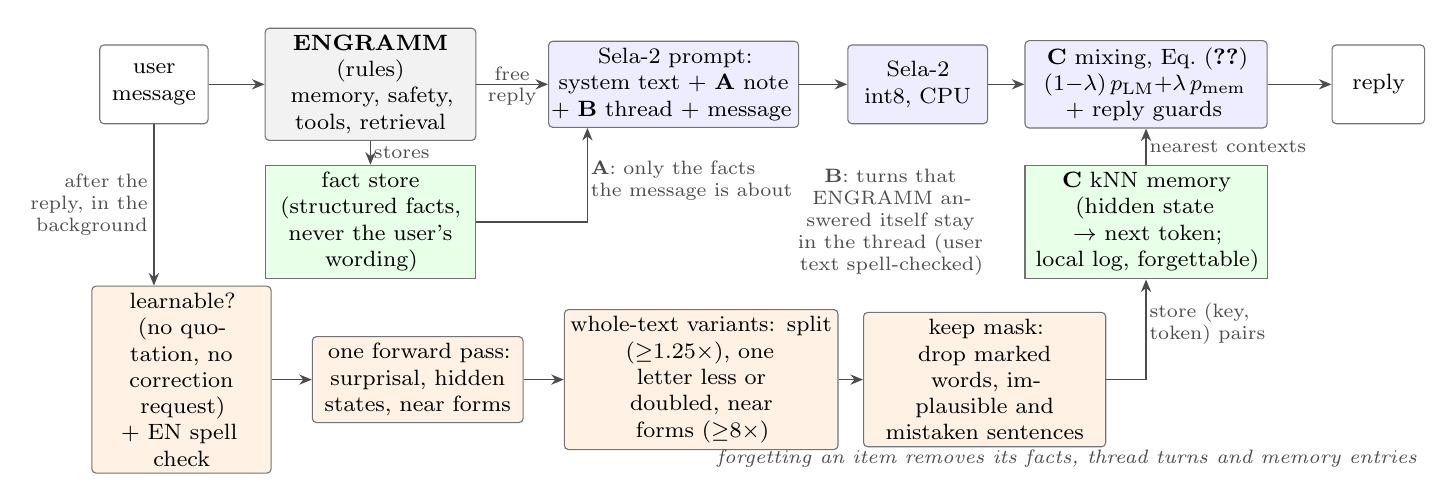
\begin{tikzpicture}[
  font=\footnotesize, x=1cm, y=1cm,
  >={Stealth[length=1.6mm,width=1.3mm]},
  box/.style={draw=black!55, rounded corners=1.5pt, align=center, inner sep=2.5pt, minimum height=10mm, text width=#1, fill=white},
  box/.default=22mm,
  eng/.style={box=#1, fill=black!5}, eng/.default=24mm,
  sela/.style={box=#1, fill=blue!7}, sela/.default=24mm,
  lrn/.style={box=#1, fill=orange!10}, lrn/.default=25mm,
  store/.style={box=#1, fill=green!9, rounded corners=0pt}, store/.default=25mm,
  lbl/.style={font=\scriptsize, text=black!70, align=center, inner sep=1pt},
  arr/.style={->, draw=black!70, line width=0.55pt}]
% row 1: the reply path
\node[box=12mm]  (msg)    at (0,0)     {user\\message};
\node[eng=25mm]  (eng)    at (2.75,0)  {\textbf{ENGRAMM} (rules)\\memory, safety,\\tools, retrieval};
\node[sela=30mm] (prompt) at (6.6,0)   {Sela-2 prompt:\\system text + \textbf{A} note\\+ \textbf{B} thread + message};
\node[sela=16mm] (lm)     at (9.7,0)   {Sela-2\\int8, CPU};
\node[sela=29mm] (mix)    at (12.6,0)  {\textbf{C} mixing, Eq.~\eqref{eq:mix}\\$(1{-}\lambda)\,p_{\mathrm{LM}}{+}\lambda\,p_{\mathrm{mem}}$\\+ reply guards};
\node[box=10mm]  (reply)  at (15.55,0) {reply};
\draw[arr] (msg) -- (eng);
\draw[arr] (eng) -- node[lbl, above] {free} node[lbl, below] {reply} (prompt);
\draw[arr] (prompt) -- (lm);
\draw[arr] (lm) -- (mix);
\draw[arr] (mix) -- (reply);
% row 2: what is kept
\node[store=25mm] (facts) at (2.75,-1.75) {fact store\\(structured facts,\\never the user's wording)};
\node[store=29mm] (knn)   at (12.6,-1.75) {\textbf{C} kNN memory\\(hidden state $\to$ next token;\\local log, forgettable)};
\draw[arr] (eng) -- node[lbl, right] {stores} (facts);
\draw[arr] (facts.east) -| node[lbl, right, pos=0.72, align=left] {\textbf{A}: only the facts\\the message is about} ($(prompt.south west)+(0.5,0)$);
\draw[arr] (knn) -- node[lbl, right] {nearest contexts} (mix);
\node[lbl, text width=27mm] at (9.35,-1.75) {\textbf{B}: turns that \mbox{ENGRAMM} answered itself stay in the thread (user text spell-checked)};
% row 3: the learning path
\node[lrn=21mm] (gate) at (0.35,-3.75)  {learnable?\\(no quotation, no\\correction request)\\+ EN spell check};
\node[lrn=25mm] (pass) at (3.35,-3.75)  {one forward pass:\\surprisal, hidden\\states, near forms};
\node[lrn=33mm] (var)  at (6.95,-3.75)  {whole-text variants: split\\($\geq$1.25$\times$), one letter less or\\doubled, near forms ($\geq$8$\times$)};
\node[lrn=29mm] (keep) at (10.55,-3.75) {keep mask: drop marked\\words, implausible and\\mistaken sentences};
\draw[arr] (msg.south) -- node[lbl, left, align=right, xshift=-1pt] {after the\\reply, in the\\background} (msg.south |- gate.north);
\draw[arr] (gate) -- (pass);
\draw[arr] (pass) -- (var);
\draw[arr] (var) -- (keep);
\draw[arr] (keep.east) -| node[lbl, right, pos=0.78, align=left] {store (key,\\token) pairs} (knn.south);
\node[lbl, anchor=north east, align=right] at (16.1,-4.6) {\textit{forgetting an item removes its facts, thread turns and memory entries}};
\end{tikzpicture}
\caption{The three learning layers. ENGRAMM, a rule-based assistant, handles every turn first and stores the user's
facts. \textbf{A}: a note built from structured facts in Sela-2's system prompt. \textbf{B}: turns that ENGRAMM answered
itself stay in Sela-2's conversation. \textbf{C}: after each reply, a learnable message is analysed by the model itself
(\cref{sec:filter}) and its kept tokens are stored as (hidden state, next token) pairs; while Sela-2 writes, the nearest
stored contexts are mixed into its next-token distribution.}
\label{fig:system}
\end{figure*}

\subsection{Sela-2, a small model trained from scratch}\label{sec:sela}

Sela-2 follows the nanochat recipe \citep{karpathy2025nanochat}, a descendant of nanoGPT \citep{karpathy2022nanogpt} and
the modded-nanogpt speedruns \citep{jordan2024modded}: 24 pre-norm decoder layers of width 1{,}024 with 8 heads, a
context of 2{,}048 tokens, rotary embeddings \citep{su2024roformer}, query--key normalisation \citep{henry2020qknorm},
RMSNorm without weights \citep{zhang2019rmsnorm}, squared-ReLU feed-forward blocks \citep{so2021primer}, two value
embedding tables, an untied output matrix and logits soft-capped at 15. Of its 503{,}316{,}938 stored parameters,
352{,}321{,}920 are used per token (value embeddings are looked up, not multiplied). Its byte-level BPE vocabulary
\citep{sennrich2016bpe} of 49{,}152 tokens averages 4.67 bytes per token on English and 4.39 on German.

Pretraining consumed 3.06\,B tokens on one H100 (4.93\,h, about 172\,k tokens/s) from FineWeb-Edu
\citep{penedo2024fineweb}, DCLM \citep{li2024dclm}, C4 \citep{raffel2020t5}, Cosmopedia, Wikipedia, PG-19
\citep{rae2020compressive} and German FineWeb2-HQ \citep{messmer2025fineweb2hq}; the final 30\pct{} of training added
chat, grounded question-answering and identity conversations (SmolTalk \citep{allal2025smollm2} and SmolTalk2,
OpenAssistant \citep{kopf2023oasst}, Dolly, SQuAD~2.0 \citep{rajpurkar2018squad2}, HotpotQA \citep{yang2018hotpotqa},
GermanRAG). Muon \citep{jordan2024muon} with Polar Express \citep{amsel2026polar} and NorMuon \citep{li2025normuon}
updated the block matrices, AdamW the rest; 657 steps of supervised fine-tuning on 78.7\,M assistant tokens followed. The
rented session lasted about 5.7\,h and cost about USD~23, including a failed first start, under a USD~25 cost limit fixed
before the run.

On a pooled zero-shot score over six tasks (HellaSwag, PIQA, ARC-Easy/Challenge, WinoGrande, OpenBookQA;
\citealp{zellers2019hellaswag,bisk2020piqa,clark2018arc,sakaguchi2020winogrande,mihaylov2018openbookqa}), measured with
one harness for all models, the base model scores 45.5 against 38.9 for GPT-2 small \citep{radford2019gpt2} (paired
bootstrap 95\pct{} CI of the difference 5.7--7.6), 42.9 for GPT-2 medium, and 39.5 and 43.5 for Pythia-160M and Pythia-410M
\citep{biderman2023pythia}; a token-level contamination audit leaves the pooled score unchanged. The chat fine-tuning
cost about four pooled points, so by a rule fixed before that comparison the app ships the interpolation
$0.7\cdot\text{base} + 0.3\cdot\text{chat}$ (``mix30'', cf.\ WiSE-FT \citep{wortsman2022wiseft}; pooled 45.7).
Quantising the chat model to int8 cost 0.001 bits per byte. Sela-2 is nevertheless a weak chat model: its free replies
are fluent but often factually wrong, and it missed several of its own preregistered chat targets (on IFEval
\citep{zhou2023ifeval} it gained at most 4.8 points over the base model, against a target of 8). We study the
personalisation of a small, imperfect model, not of a capable assistant.

\subsection{The host assistant}\label{sec:host}

Sela-2 runs inside ENGRAMM, an offline desktop assistant that itself uses no neural network: it answers factual
questions from a local Wikipedia/Wikidata pack, keeps a rule-based store of what the user tells it, handles safety,
tools and clarifying questions, and forgets on request. ENGRAMM handles each turn first. Its memory, safety and tool
replies are shown as they are; answers with sources are rewritten by Sela-2 and shown only if every number and name in
the rewrite occurs in a cited source; small talk, writing requests and open questions receive Sela-2's free reply, which
is what the learning layers affect. The int8 model runs on NumPy with numba kernels; in the measurements from \S8 on it wrote
\stat{tokps.min}--\stat{tokps.max} tokens per second (F arms) on GitHub-hosted CI runners.

\subsection{Three learning layers}\label{sec:layers}

\paragraph{A: the fact note.} ENGRAMM's fact store holds structured facts extracted from statements (``My dog is called
Rex'' becomes an owned pet \emph{dog} named \emph{Rex}). Layer A renders up to eight of them into a note at the end of
Sela-2's system prompt. The note is built from the structured facts, never from the user's wording, so a typo in the
original message cannot enter it; facts about other people, about the past and negated facts are not shown, and the
newest value of a single-valued fact wins. Since \S10 of the preregistration the note is written in the third person
(``About the user (\ldots{} facts about the user, not about you; use them only when they help): The user's name is Sam.
The user lives in Leeds. The user's dog is called Rex.''); since \S12 it holds only the facts the current message is
about (\cref{sec:intrusion}). Two guards act on every free reply: sentences in which Sela-2 states a user fact as its
own (``I live in Leeds.'') are removed, and so are sentences that repeat the note.

\paragraph{B: the thread.} Turns that ENGRAMM answers itself, such as a statement it stores, stay in Sela-2's
conversation history; English user text first passes through ENGRAMM's spell checker. Before this layer existed,
Sela-2 recommended New York to a user who had just said they were planning a trip to Italy.

\paragraph{C: the language memory.} For every token $t_j$ of a learned message, the memory stores a key and the value
$t_j$. The key is Sela-2's normalised final hidden state at the position that predicts $t_j$, projected to 128
dimensions by a fixed Gaussian random matrix \citep{johnson1984extensions} and scaled to unit length. While Sela-2
writes, the current hidden state is projected likewise, the $K = 16$ stored keys with the highest cosine similarities
$s_i$ are retrieved, and
\begin{align}
p(w) &= (1-\lambda)\,p_{\mathrm{LM}}(w) + \lambda\,p_{\mathrm{mem}}(w), \label{eq:mix}\\
p_{\mathrm{mem}}(w) &\propto \textstyle\sum_{i:\,t_i = w,\; s_i \geq \theta} e^{(s_i - s_{\max})/\tau},\notag\\
\lambda &= \lambda_{\max}\,\textstyle\min\!\big(1, \max\!\big(0, \frac{s_{\max}-\theta}{1-\theta}\big)\big),\notag
\end{align}
with $\lambda_{\max} = 0.10$, similarity floor $\theta = 0.90$ and $\tau = 0.01$, chosen on development users. The memory
thus has no influence unless a stored context is very close, and never more than a tenth of the probability. Proposals
that the admission filter would judge to be misspellings are removed from $p_{\mathrm{mem}}$ before mixing. Messages are
learned in the background after the reply, holding the model lock only for single forward passes; the memory keeps at
most 20{,}000 entries (about 1{,}000 messages), oldest out first.

\paragraph{Forgetting.} Thread turns and memory entries that stem from a message ENGRAMM stored carry the identifier of
that memory item and are removed with it. Emptying the memory, the reset on the app's learning page, or ``forget
everything you learned'' clears the whole language memory, an append-only text log plus a derived cache of keys.

% ======================================================================================================================
\section{Error-aware admission to the memory}\label{sec:filter}

The memory learns what follows what in the user's messages, so a misspelt word would be stored as a likely continuation
and boosted whenever a similar context recurred. The filter (\cref{alg:filter}) keeps mistakes out with the model's own
knowledge of the language. Its central operation compares the likelihood of the \emph{whole} message, including the end
of the turn, with and without a small change. Token-level comparisons miss many real mistakes because a mistake changes
the tokenisation: \emph{alot} must be compared with the two tokens \emph{a lot}, and \emph{wiederrum} with the single
token \emph{wiederum}. Scoring a variant costs only the suffix from its first changed token: the key/value cache is
rewound to that position, and variants are scored from the last changed position to the first, so earlier text is never
recomputed (rewound scores matched full passes to within \stat{r15.drift} nats). The analysis runs in the background; in
the development probe of the final code, which scores more variants than the app, it took \stat{r15.analyse.mean}\,s per
message on average (at most \stat{r15.analyse.max}\,s) on a CI runner.

\begin{algorithm}[t]
\caption{Admitting one user message to the memory (\cfile{engramm/lm/sela_learn.py}).}
\label{alg:filter}
\footnotesize
\begin{algorithmic}[1]
\If{$m$ has $<4$ words or $>800$ characters, asks to correct, rewrite or translate, or quotes text}
  \State \Return (nothing is learned)
\EndIf
\State if $m$ is English, fix spelling slips with ENGRAMM's spell checker
\State one pass of Sela-2 over $m$ as a user turn: surprisal $n_j$ and hidden state of each token $t_j$
\State \textbf{near forms:} $t_j$ is \emph{near} if one of the 20 likeliest tokens at $j$ is $\geq 8\times$ likelier than $t_j$ and nearly the same string (edit distance $\leq 2$, or same first three letters and lengths within 3)
\For{up to 8 words $w$ ($\geq 4$ letters), most surprising first}
  \State \textbf{split variants:} splits of $w$ into two single tokens (\emph{alot} $\to$ \emph{a lot})
  \State \textbf{letter variants} (3 most surprising words of $\geq 5$ letters, $\geq 6$ nats): one letter removed or one consonant doubled
  \State score a variant only if the model prefers it at its first changed token, or (letter) it needs fewer tokens
  \State mark $w$ if a variant makes the whole message $\geq 1.25\times$ (split) or $\geq 8\times$ (letter) likelier, unless it only drops the first letter or a non-doubled last letter (\emph{shape rule})
\EndFor
\State \textbf{confirm} up to 6 near tokens with $n_j \geq 6$ nats: the near form must make the whole message $\geq 8\times$ likelier
\State \textbf{keep mask:} drop words with a near token or a mark; drop sentences with median surprisal $> 6.5$ nats; drop every sentence with a marked word or a confirmed near form
\State \Return (key, token) pairs of the kept tokens
\end{algorithmic}
\end{algorithm}

\paragraph{Why drop whole sentences.} A sentence built around a mistake teaches its structure even without the wrong
word: from \emph{Gestern ich habe gegangen zum B\"acker} the memory would still learn that \emph{ich} follows
\emph{Gestern}. A clear mistake therefore removes its sentence. A near form that is merely likelier at its own position
is too weak a signal for this (in a development probe it would have discarded 246 of 320 correct sentences; \S8 of the
preregistration), so it removes its sentence only when the whole message confirms it.

\paragraph{What the filter cannot see.} Grammar mistakes made of correct words (\emph{ich habe gegangen},
\emph{wegen dem Wetter}) are caught only when a near form of one token makes the whole message much likelier, and a
missing letter is not tried. The filter also cannot know whether an unusual word is a mistake or the user's choice;
every check trades stored mistakes against discarded correct text (\cref{sec:letter}).

\paragraph{Choosing the letter rule in advance.} On new users the letter check also flagged correct words: British
\emph{favourite} (the model prefers \emph{favorite}), inflections (\emph{parts} $\to$ \emph{part}), German declension. A
first counter-measure, requiring the variant to be likelier also as a word on its own, let real mistakes through
(\emph{Packet} is a valid English word). We then replayed 18 candidate rules from the recorded traces of one development
probe: no outside check, the word alone, or the word in a fixed sentence (``I wrote the word \_\_ down.''), at 0, 1, 1.5
or 2.08 nats, each with and without the shape rule. The selection criterion was fixed before the results were
inspected: admissible are rules that, over four user sets (real development users and the consumed synthetic users of
\S7, \S9, \S10), store no more injected mistakes than the previous rule without outside check; among them, the highest
memory gain on the real development users wins.

% ======================================================================================================================
\section{Evaluation protocol}\label{sec:protocol}

\paragraph{Preregistration.} Each version was registered in a section (\S7--\S12) of \file{docs/PREREG_SELA2.md},
committed before the commit that triggered its measurement; the measurement ran on GitHub Actions on that commit's
code, and the workflow committed the results (\cref{app:timeline}). Apart from whitespace, each section's registered
text is identical in its triggering commit and the final document; results were appended as subsections. Development
used only consumed users (those of earlier measurements) and real development users; the development probe refuses the
synthetic \S8 test file and all real test files. Before the first measurement, four rounds of code review by separate
AI agent instances that had not written the code (five reviewers in the first), with each finding checked by a second
such reviewer, found 85 defects, all fixed before anything was measured. The sequence from the
registration of \S7 to the decision of \S12 took place on 19 October 2026 (00:28--18:59 UTC).

\paragraph{Synthetic users.} Each synthetic group (\S7--\S10) has 20 English and 20 German users generated by a fixed
script with a new seed and new names, cities, pets, dishes and hobbies. A user writes eight teaching messages: four fact
statements (name, city, pet and its name, favourite dish) and four messages about a hobby; three of the latter are
followed by a sentence with a typical mistake from a fixed list of 12 English and 12 German mistakes: misspellings
(\emph{freind}, \emph{definately}, \emph{Standart}, \emph{Packet}), merged words (\emph{alot}, \emph{garnicht}) and
grammar (\emph{she go}, \emph{he don't}, \emph{ich habe gegangen}). Two further hobby sentences are held out (never
taught, free of mistakes). Each group is built from 10 hobby scripts (five per language), each shared by four users
who differ only in facts and mistakes, so a group has 20 distinct held-out sentences, not 80.

\paragraph{Real users.} \S11 and \S12 use real people's messages to a chatbot from WildChat-1M
\citep{zhao2024wildchat} at a fixed revision (\cref{app:selection}). A user is one hashed IP address within one language
(English or German), restricted to conversations not flagged as toxic or redacted. Messages count if they read as plain
prose (20--300 characters, no code, links or markup), in time order and without near copies; users with six such
messages qualify, the first four are taught and the next two held out. Development and test users are separated by a
hash of the hashed IP; 20 users per language and split were drawn with a fixed seed, and the selection (identifiers and
hashes only) was committed before anything was measured on them. Facts, injected mistakes and probes are added as for
synthetic users. Whether the app would learn a message was not used for selection; in the development set
\stat{r15.learnable} messages were learnable, most others contain quotations.

\paragraph{Arms, probes and criteria.} After teaching, each probe is asked in a new conversation in three arms with the
same seed: \textbf{off} (no learning; the app before \S7), \textbf{F} (layers A and B) and \textbf{FK} (A, B and C). Each
arm starts from the state after teaching; probes are not learned. A user has four \emph{fact probes} whose natural answer
uses one fact (``What should I cook tonight? One idea, please.''), two \emph{error probes} inviting the correct form of
two of their mistakes (``Write one sentence about learning a lot in a short time.'') and one hobby probe; \S12 adds two
neutral requests and uses blind-written fact probes. The 100 fixed prompts of Sela-2's chat evaluation (60 English, 40
German) are also run through the app in each arm after teaching the first test user. \Cref{tab:criteria} defines the
criteria. From \S7 on, A+B were to be switched on if L1, L2, L2b and L4 held for F, and C additionally if L2, L2b and L4
held for FK and L3 and L5 held; a decision required all 40 users, all app arms, no crashed reply and an L1 coverage of at
least 50\pct. Later sections restricted the rule to the component being decided (\cref{app:rules}).

\begin{table}[t]
\centering
\footnotesize
\setlength{\tabcolsep}{3pt}
\caption{Criteria; thresholds compare an arm with \emph{off} on the same users and seeds.}
\label{tab:criteria}
\begin{tabularx}{\columnwidth}{@{}lXl@{}}
\toprule
& Definition & Threshold \\
\midrule
L1 & \emph{Fact use}: fact probes whose reply contains the fact (or a listed inflection), on probes Sela-2 answered in all arms (valid only if $\geq 50\pct$ of them) & F$-$off $\geq{+}15$ \\
L2 & \emph{Copied mistakes}: replies containing one of the user's injected wrong forms & $\leq$ off${+}2$ \\
L2b & \emph{Role confusion}: replies stating a user fact as Sela-2's own (fixed patterns) & $\leq$ off${+}2$ \\
L3 & \emph{Memory gain}: relative reduction in bits per byte on held-out messages, memory vs.\ none & $\geq 1\pct$ \\
L4 & \emph{App problems}: app prompts with a detected problem (wrong language, identity error, echo, cut-off, role leak, loop, empty, crash) & $\leq$ off${+}2$ \\
L5 & \emph{Writing speed} after reading the prompt, FK/F & $\geq 0.85$ \\
L6 & \emph{Intrusion} (\S12): probe replies naming a fact the probe did not ask for; app replies naming the taught user's facts & $\leq 10\pct$; $\leq 3$ \\
\bottomrule
\end{tabularx}
\end{table}

\paragraph{Uncertainty.} Registered decisions compare point estimates with thresholds, and we report them as registered.
We add 95\pct{} intervals that were not part of any registration: Wilson intervals \citep{wilson1927probable} for
proportions (treating replies as independent; for L1, a bootstrap over users moves the interval ends by at most
\stat{l1boot.maxdiff} points), and for
L3 a percentile bootstrap \citep{efron1993bootstrap} with 10{,}000 replicates over the independent units, users for real
groups and hobby scripts for synthetic groups. With 10 clusters the synthetic intervals are approximate.

% ======================================================================================================================
\section{Results}\label{sec:results}

\begin{table*}[t]
\centering
\footnotesize
\setlength{\tabcolsep}{4pt}
\caption{All registered measurements, 40 fresh users each. L1: F$-$off in points on 160 fact probes (\S12: the 116 that
Sela-2 answered in all arms; off was 0\pct{} in every run), with 95\pct{} Wilson interval. L2, L2b: replies F / FK out of 280 per arm (\S12: 360); off was 0 in every run. L3: \% with 95\pct{}
cluster-bootstrap interval. L4: app prompts with a problem, F / FK (off). L5: writing speed FK/F. L6: \% of Sela-2's probe
replies (291 per arm), F / FK. $^{\dagger}$See \cref{sec:overview}.}
\label{tab:registered}
\begin{tabular}{@{}llllllllll@{}}
\toprule
& Users & L1 F$-$off [95\pct{} CI] & L2 & L2b & L3 [95\pct{} CI] & L4 & L5 & L6 & Decision \\
\midrule
\tablebody{tab_registered}
\bottomrule
\end{tabular}
\end{table*}

\subsection{The sequence of measurements}\label{sec:overview}

\Cref{tab:registered} lists every registered measurement. The \textbf{first version} (\S7) showed the facts as an earlier
first-person user turn (``My name is Sam. My dog is called Rex.'') and used an older filter with stronger mixing
($\lambda_{\max}{=}0.30$, $\theta{=}0.80$, $\tau{=}0.05$). Fact use rose from 0 to 52.5\pct, but Sela-2 repeated the fact
lines as its own in 7 replies per arm (\emph{Ich hei\ss{}e Lea.}), the memory copied \emph{alot} and \emph{garnicht} into 6
replies, gained only 0.55\pct{} and slowed generation to 0.79 of the off arm. By the rule, all layers stayed off. The
\textbf{second version} (\S8) moved the facts into a labelled note with a role-confusion guard, introduced the filter of
\cref{sec:filter}, and took the mixing setting from a grid on the consumed \S7 users. On 40 fresh users it met every
criterion, and all layers were switched on.

\S9 compared two note forms on new users: third-person sentences raised fact use to 44.4\pct{} against 20.0\pct{} for
labels (of 160 fact probes; German 40.0\pct{} against 13.8\pct{} of 80). But the registered rule adopted the sentence form only if that run
\emph{also} met the criteria of layer C, and C missed L3 (0.78\pct). The sentence form was not adopted ($^{\dagger}$), and
C was switched off again. The rule was badly built: it tied a decision about the note to a criterion of the memory,
which never sees the note (L3 is identical in both arms). We did not override it; \S10 repeated the comparison on 40
further users with a rule about the note alone. Sentences won again (+34.4 against +23.8 points) and became the default;
the memory gained 0.09\pct{} and stayed off. \S11 measured the memory on real users and switched it on; \S12 tested the
relevance filter.

\paragraph{Facts.} Moving the facts from a first-person turn into a note removed role confusion (L2b: 7 replies per arm
in \S7, 0 in every later run). Writing the note as sentences instead of labels raised fact use on two fresh groups by 24.4 and
10.6 points; the change was motivated by development runs in which, with labels (\emph{Name: Lea; Hund: Bruno}), the
small model often took the user's name for the pet's. Fact
use was lower in German than in English in most runs (27.5\pct{} against 41.2\pct{} of 80 each with sentences in
\S10). L1 counts any
mention of a fact, fitting or not; that weakness led to \S12.

\subsection{Where the mistakes went}\label{sec:mistakes}

\begin{table}[t]
\centering
\footnotesize
\setlength{\tabcolsep}{3.5pt}
\caption{Fate of the 120 injected mistakes per registered measurement, read from the memory itself, and FK replies that
contained an injected wrong form (280 per run; \S12: 360). Both runs of \S9, \S10 and \S12 teach the same memory; their
copies are given as labels / sentences and filter on / off. Spell checking applies to English only.}
\label{tab:errors}
\begin{tabular}{@{}lrrrrr@{}}
\toprule
& spell- & not & & & copied \\
Measurement & checked & learnable & filtered & stored & (FK) \\
\midrule
\tablebody{tab_errors}
\bottomrule
\end{tabular}
\end{table}

\Cref{tab:errors} follows each injected mistake. From \S8 on, 4--10 of 120 mistakes reached the memory per measurement,
against 23 with the first filter. On the \S7 users used for development, the code measured in \S8 had stored none
(\cref{app:dev}): a gap between development and test for a filter whose thresholds were set on those users. The leaks
are specific. A probe of the final code on the real development users, which unlike the app does not spell-check
English, stored \stat{r15.stored} mistakes: \stat{r15.stored.en} English misspellings that the app's spell checker
corrects first (\stat{r15.en.forms}) and \stat{r15.stored.de} of \stat{r15.n.de} German mistakes. For \emph{Packet} and
one \emph{wiederrum} the correct forms made the message 2.01 and 2.07 nats likelier, just short of $\log 8 \approx 2.08$;
the other \emph{wiederrum} was never checked because its message held three more surprising words; \emph{Rhytmus} lacks a
letter, which is not tried; and for \emph{garnicht} the split made that message less likely. F replies never contained an
injected mistake. Of the 2{,}400 FK replies of \S8--\S12, four did: two reproduced a stored \emph{garnicht}, while in the
other two the memory had filtered the sentence and \emph{ich habe gegangen} arose without a stored copy.

\subsection{Why the memory's gain fell: lexical reuse}\label{sec:reuse}

\begin{figure*}[t]
\centering
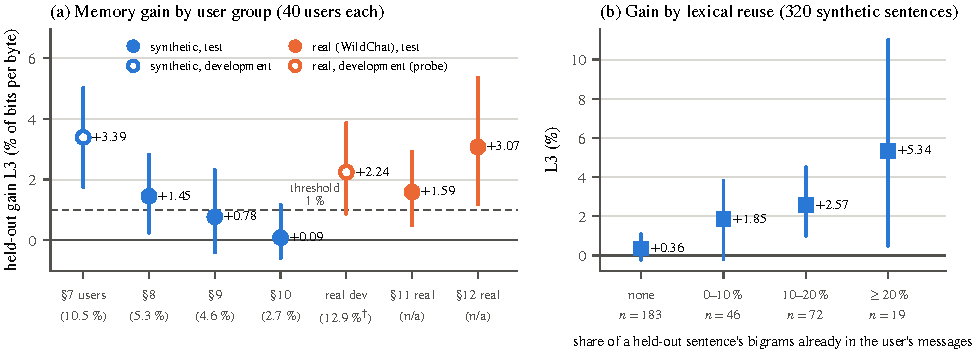
\includegraphics[width=0.94\textwidth]{figures/fig_l3_reuse.pdf}
\caption{(a) Memory gain L3 on held-out messages by user group, with 95\pct{} bootstrap intervals (over hobby scripts for
synthetic groups, over users for real groups). In parentheses: share of the held-out sentences' word pairs (bigrams)
already present in the same user's taught messages. $^{\dagger}$Recorded in the preregistration (\S11); the texts are not
in the repository, so it cannot be recomputed here. The real development value comes from a development probe, the
others from app measurements. (b) Gain over the 320 synthetic held-out sentence scores, binned by bigram reuse;
cluster-bootstrap intervals over hobby scripts.}
\label{fig:reuse}
\end{figure*}

The memory gained \stat{G.dev7}\pct{} on the \S7 users during development but only \stat{G.g8}, \stat{G.g9} and
\stat{G.g10}\pct{} on the three fresh synthetic groups (\cref{fig:reuse}a). The mixing setting does not explain this: on the
consumed \S9 and \S10 users, the best of 60 settings of $(\lambda_{\max}, \theta, \tau)$ reached \stat{grid.best.g9} and
\stat{grid.best.g10}\pct, against \stat{grid.app.g9} and \stat{grid.app.g10}\pct{} for the app's setting, and larger
memory shares only hurt, down to \stat{grid.worst.g10}\pct{} (\cref{tab:grid,fig:grids}).

The evidence points to the test sentences: a memory of someone's wording can only help where they reuse it. For every
held-out sentence we measured the share of its lower-cased word bigrams that already occur in the same user's taught
messages. Pooled per group, this share was \stat{reuse.s7}\pct{} for the \S7 users and \stat{reuse.s8}, \stat{reuse.s9}
and \stat{reuse.s10}\pct{} for the three test groups, the same order as their gains. Over all 320 synthetic sentence
scores, the gain rises with reuse (\cref{fig:reuse}b, \cref{tab:reuse}) from \stat{bin.none}\pct{} for sentences
sharing no word pair with the user's messages to \stat{bin.ge20}\pct{} for those sharing a fifth or more; the
per-sentence rank correlation is $\rho = \stat{rho}$ (95\pct{} CI \stat{rhoci}). The pattern holds within three of four
groups: sentences with reuse gained \stat{wp.s7}, \stat{wp.s8} and \stat{wp.s9}\pct, those without \stat{wz.s7},
\stat{wz.s8} and \stat{wz.s9}\pct{} (\S7, \S8, \S9); in \S10 the \stat{wpn.s10} sentences with reuse gained nothing
(\stat{wp.s10}\pct). How much the held-out sentences reused the teaching messages was our choice when writing them, not a
property of users, and with only 10 hobby scripts per group a few scripts decided it.

Real users reuse more of their wording: on the 40 real development users, 12.9\pct{} of the held-out messages' word
pairs occurred in their earlier messages (recorded in the preregistration). On the deciding test with 40 real users, the
memory's gain was \stat{G.g11}\pct{} (95\pct{} CI \stat{Gci.g11}), and it met all criteria of layer C: one
copied mistake (limit 2), no role confusion, writing speed 0.967 of F. It was switched on. On 40 further real users (\S12,
where it was reported but not decided on) it gained \stat{G.g12}\pct{} (\stat{Gci.g12}). The intervals are wide: 40
users cannot establish with confidence that the deciding gain of 1.59\pct{} lies above the 1\pct{} threshold.

\subsection{Choosing the letter rule}\label{sec:letter}

\begin{figure*}[t]
\centering
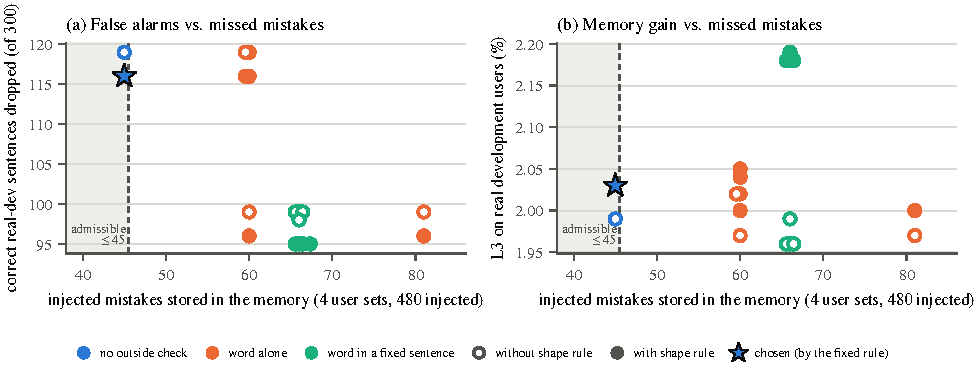
\includegraphics[width=0.94\textwidth]{figures/fig_letter_rules.pdf}
\caption{The 18 letter rules of development probe round 14, replayed from the same traces. Horizontal: injected mistakes
stored, summed over four user sets (480 injected). (a) Correct real-development sentences dropped whole (lower is
better). (b) Memory gain on the real development users (higher is better; note the narrow range). Rules left of the
dashed line were admissible under the criterion fixed in advance; the star marks the selected rule. Rules with identical
results are drawn slightly apart. The probe does not run the app's English spell checker, so stored counts include
English misspellings that the app corrects first.}
\label{fig:letter}
\end{figure*}

\begin{table}[t]
\centering
\footnotesize
\setlength{\tabcolsep}{3pt}
\caption{Letter rules (excerpt; all 18 in \cref{tab:letterall}): L3 on real development and consumed \S7 users,
mistakes stored over four sets, correct real-development sentences dropped (of \stat{lr.ncorrect}). The earlier fix
is the word-alone check of commit 63123a5.}
\label{tab:letter}
\begin{tabular}{@{}lrrrr@{}}
\toprule
& L3 real & L3 \S7 & & \\
Rule & dev (\%) & (\%) & stored & dropped \\
\midrule
\tablebody{tab_letter}
\bottomrule
\end{tabular}
\end{table}

\begin{table*}[t]
\centering
\footnotesize
\caption{\S12 on 40 further real test users with blind-written fact probes: relevance filter on (decides) and off
(comparison on the same users, probes and seeds). Counts are replies; 95\pct{} Wilson intervals in brackets.}
\label{tab:s12}
\begin{tabular}{@{}llll@{}}
\toprule
Criterion & Filter on & Filter off & Threshold \\
\midrule
\tablebody{tab_s12}
\bottomrule
\end{tabular}
\end{table*}

\Cref{fig:letter} shows the trade-off in the letter check. The fixed-sentence checks at every threshold and the
word-alone checks from 1.5 nats reduced false alarms, from 116--119 to 95--99 correct sentences dropped on the real
development users, but every outside check let more injected mistakes through: \stat{lr.outside.minstored}--\stat{lr.outside.maxstored} stored against \stat{lr.baseline} without one
(\cref{tab:letter}). Only the two rules without an outside check were admissible, and the criterion selected the shape
rule, which stores no more mistakes and drops fewer correct sentences (\stat{lr.chosen.dropped} instead of 119). The
earlier counter-measure (word alone, above 2.08 nats) stored 81. The gains of all 18 rules lie within 0.23 points, far
less than the uncertainty of L3; the choice was made on mistakes, as intended.

The filter as a whole has a price. In a probe of the final code on the real development users (round 15, in which a
mistake sentence no longer merges with a real message that lacks closing punctuation, so that 353 correct sentences are
counted instead of 300), it dropped
\stat{r15.R2_app.dropped} correct sentences whole, against \stat{r15.R0_none.dropped} with word-level filtering alone, and
the memory gained \stat{r15.R2_app.L3}\pct{} instead of \stat{r15.R0_none.L3}\pct; in exchange, the error-carrying
sentences that still contributed tokens fell from \stat{r15.R0_none.errpart} to \stat{r15.R2_app.errpart}. Not learning a
user's mistakes cost about 30\pct{} of what the memory could gain from those users.

\subsection{Unrequested facts and the relevance filter}\label{sec:intrusion}

L1 counts every mention of a fact, whether it fits or not, and many did not fit: asked what to do with the dog in a
free afternoon, Sela-2 answered \emph{Niklas und Bruno machen gerne gemeinsam Lasagne} (``Niklas and Bruno like making
lasagne together''). Counted afterwards on consumed measurements, \stat{intr.v4s}--\stat{intr.real}\pct{} of Sela-2's
probe replies in arm F named a fact the probe had not asked for, and 10--15 of the 95--96 app replies named the taught user's
facts, often as Sela-2's own (``Hi!'' $\to$ ``Hi! I like to play with my dog Rex.''; \cref{tab:intrusionbefore}). Without
the note the rate was zero. Large assistants show the same failure \citep{hu2026opbench,feng2026rpeval}.

\S12 tested a deliberately simple remedy: the note shows only the facts the message is about. A fact qualifies if the
message names its value (\emph{Rex}, \emph{Leeds}), or its subject through short cue lists per category and language
(\emph{cook}, \emph{dinner}, \emph{Rezept} for the dish; \emph{dog}, \emph{pet}, \emph{Hund} for the pet;
\emph{sign-off}, \emph{e-mail}, \emph{Gru\ss{}formel} for the name; \emph{near me}, \emph{in der N\"ahe} for the city), or
if it asks what Sela-2 knows about the user (then all are shown). The role-confusion guard still checks all facts. The
cue words were frozen in a commit (96e9897) before the test probes existed. The probes were then written by a separate
AI agent instance from a description of the four fact intents and of neutral requests, without access to the
repository, the filter or its cue words: six formulations per fact and twelve neutral requests per language,
committed with the registration. Each of 40 further real test users received one blind probe per fact and two neutral
requests. We read the probes after they arrived and changed nothing. Measurement 1 (filter on) decided; measurement 2
(filter off) ran on the same users, probes and seeds.

With the filter, Sela-2 used the facts exactly as often where they were asked for (\stat{s12.L1k.on} fact probes in both
runs) but almost never volunteered them: \stat{s12k.on.F} probe replies named an unrequested fact, against
\stat{s12k.off.F} without the filter, and 1 against 12 of 96 app replies (\cref{tab:s12}). The filter met every registered
criterion and became the default. Two qualifications. First, the app count of L6 was recorded for every reply during the
measurement, but the app evaluation's summary did not add it up; we counted it afterwards from the same recorded replies,
with no new measurement, and only that entry changed (commit 2edd391). Second, cue words fail in both directions: the
remaining app cases (one prompt in F, two in FK) were requests to summarise a text that was not about the user, in
which a cue word showed a fact (\emph{email} the name, German \emph{Stadt} the city), and blind English probes without a
cue word received no note, so English fact use was one probe lower with the filter
(\stat{s12.L1en.on} against \stat{s12.L1en.off} of \stat{s12.L1enn}; German \stat{s12.L1de.on} against
\stat{s12.L1de.off} of \stat{s12.L1den}). On the blind probes, ENGRAMM answered 27.5\pct{} of the
fact probes itself, so L1 rests on the 116 that Sela-2 answered in all arms.

\paragraph{Cost.} The memory slowed writing by 2--4\pct: L5 lay between 0.963 and 0.975 in all registered measurements
from \S8 on (0.79 for the first version, under an older definition that included reading the prompt). The analysis runs
after the reply and blocks a new reply for at most one forward pass. Eight teaching messages produced on average
\stat{entries.min}--\stat{entries.max} memory entries per user from \S8 on (\stat{entries.s7} with the first filter),
each a 128-dimensional key (cached on disk in half precision) and a token id.

% ======================================================================================================================
\section{Discussion}\label{sec:discussion}

\paragraph{What we think generalises.} A personal memory needs a policy for what it may learn, not only for what it
retrieves. A model's own likelihood, compared on whole texts, is a cheap, language-independent basis for such a policy
and catches what token-level checks cannot (merged and split words). Its price is real: on our real development users,
the filter discarded two fifths of the correct sentences and about 30\pct{} of the achievable gain. Where to draw the line
is a product decision that a criterion fixed in advance can make explicit, as for our letter rule. Second, showing a
small model every fact it knows makes it talk about the user; choosing facts by relevance before generation solved this
here with simple, frozen cue words.

\paragraph{Lessons about synthetic test users.} Synthetic users are convenient and safe, and we still recommend them for
early development, but they misled us in three ways. Properties that decide the outcome can be set unknowingly by
whoever writes the data: our choice of how much held-out sentences reused the users' wording, not the method, most
likely drove the decline from \stat{G.dev7}\pct{} to \stat{G.g10}\pct; such properties should be measured and reported with the results.
``40 users'' may hide far fewer independent units: our synthetic groups had 10 hobby scripts each, and resampling users
instead of scripts would have shown intervals only about half as wide (the script intervals are
\stat{ciratio.min}--\stat{ciratio.max} times wider). And the development set shapes the method: zero stored mistakes on
the \S7 development users became 4--10 on each fresh group. A modest sample of real users changed our
conclusion about layer C.

\paragraph{Lessons about preregistration.} The registrations prevented us from rescuing the sentence note in \S9 after the
fact, although its advantage was large, and they made the repetition in \S10 necessary and convincing; they also
exposed our own errors. The \S9 rule shows the design lesson: a decision should depend only on the criteria of the
component it decides. Preregistration does not make small samples large: several decisions passed or failed a point
threshold by less than the uncertainty of 40 users, and a registered rule makes such decisions consistent, not certain.

% ======================================================================================================================
\section{Limitations}\label{sec:limitations}

\begin{itemize}
\item \textbf{One model, one application, two languages.} All results concern Sela-2 (mix30) inside ENGRAMM in English
and German; a larger model might use facts better and copy fewer mistakes.
\item \textbf{Small samples.} 40 users per measurement; the synthetic groups contain only 10 independent hobby scripts.
Several decisions rested on point estimates close to their thresholds.
\item \textbf{Synthetic facts and mistakes.} Even for real users, facts and mistakes were synthetic: four fact statements
and three appended sentences from one fixed list of 24 mistakes, the same list in every group. The filter's thresholds
were developed on the mistake types later tested, and we did not measure how many of the real users' own, natural
mistakes entered the memory.
\item \textbf{What L1 and L3 do not measure.} L1 counts mentions of facts, not whether they help; L6 covers one way of being
unhelpful. L3 measures how well the model predicts a user's own held-out messages, which need not mean better replies
\citep{wang2023knnlm}. We did not measure answer quality or helpfulness, and no human rated any reply.
\item \textbf{The filter's errors.} It discards many correct sentences and still stores some mistakes; grammar mistakes of
correct words, missing letters and mistakes that are valid words in the other language largely escape it.
\item \textbf{Cue words} were frozen before the blind probes existed but miss phrasings and misfire on requests that are
not about the user, as both happened in \S12.
\item \textbf{Our own mistakes.} The \S9 rule coupled unrelated criteria; a development counter-measure (the word-alone
check) let real mistakes through before the letter-rule comparison replaced it; the \S12 app intrusion count was summed
only after the measurement; and some counts in the project's prose documents differ from the result files
(\cref{app:discrepancies}). We report the result files throughout.
\item \textbf{Speed of the process.} The whole sequence took one day, with most implementation done by an AI coding agent
(\cref{sec:ethics}). Registrations precede their measurements in the version history, but no external party reviewed
them before the measurements.
\end{itemize}

% ======================================================================================================================
\section{Ethics, privacy and AI assistance}\label{sec:ethics}

\paragraph{Real user data.} WildChat-1M consists of conversations with a chatbot whose users consented to their
collection for research \citep{zhao2024wildchat}; it is released under the ODC-By licence and identifies users only by hashed IP addresses. We
used English and German conversations not flagged as toxic or redacted. The repository stores only the selection
(conversation hashes, turn identifiers, SHA-256 and length of each message); the texts are reassembled from the fixed
public revision inside the CI job of a measurement and checked against their hashes. Result files keep real messages
only as hash and length, and every run of four or more words written by a real user is removed from stored replies and
facts. This paper quotes no text written by a real user: quoted user messages and facts are synthetic or
blind-written probes, and quoted replies are Sela-2's.

\paragraph{The system.} What layers A, B and C learn stays on the user's computer and can be deleted exactly. The
relevance filter and the guards reduce, but do not eliminate, the risk that personal facts surface in unexpected
contexts. Sela-2's weights are not distributed; parts of its training data were generated by models whose licences
impose conditions on redistribution, which would first have to be met.

\paragraph{AI assistance.} The code, the measurement workflows and most of the documentation in the repository were
written by an AI coding agent (Claude, by Anthropic) under the author's direction: up to the commit that applied
the last decision (68a2782), 806 of 859 commits are attributed to the agent and 49 to automated CI workflows. The code
reviews of \cref{sec:protocol} and the blind probes of \S12 (written without access to the repository) were also made
by AI agents: separate instances of the same model, which had not written the code. The author set the goals, the
constraints and the budget and is responsible for the claims. This paper was drafted with
AI assistance from the repository's records; every number in it is computed from, or quoted from, repository files
(\cref{app:provenance}).

% ======================================================================================================================
\section{Conclusion}\label{sec:conclusion}

A small language model trained from scratch for about USD~23 can learn from its user on the user's own computer: a note
of the user's facts, shown only when the message is about them, and a memory of the user's wording guarded by the
model's own judgement of what looks like a mistake. Measured under preregistration on fresh users, the facts were used,
the user's mistakes were rarely stored and almost never repeated, and the memory helped real users modestly. The most
transferable result concerns evaluation: a memory-based personalisation can appear to stop working simply because the
test sentences written for it stopped reusing the users' words, and only real users revealed this. Preregistration did
not make 40 users enough to settle every question, but it made each answer, and each of our mistakes, visible.

\paragraph{Reproducibility statement.} Every number is computed by \file{paper/make_figures.py} from result files in the
project repository or quoted from them (\cref{app:provenance}). Rerunning the measurements requires the Sela-2 weights
(\file{sela2-mix30.npz}, not public), ENGRAMM's lite knowledge pack, the GitHub Actions workflows
\file{sela2_learn_eval.yml} and \file{sela2_learn_probe.yml}, and for real users the public WildChat-1M revision 7d6490e.
Synthetic users are generated deterministically by \file{experiments/sela2_learn_data.py}; the real-user selection is in
\file{data/sela2/learn_real_ids.json}. Code and weights are available from the author on request.

% ======================================================================================================================
{\small
\bibliographystyle{abbrvnat}
\bibliography{references}
}

% ======================================================================================================================
\onecolumn
\appendix

\section{Provenance of tables and figures}\label{app:provenance}

Paths are relative to the repository root. ``Script'' is \file{paper/make_figures.py}; it reads only the files named,
writes \file{paper/generated/} and \file{paper/figures/}, and uses a fixed bootstrap seed per quantity.

\begin{small}
\noindent\begin{tabularx}{\linewidth}{@{}lY@{}}
\toprule
Item & Source files \\
\midrule
\Cref{fig:system}, \cref{alg:filter}, Eq.~\eqref{eq:mix} & \file{engramm/lm/sela_learn.py}, \file{engramm/lm/sela_chat.py}, \file{engramm/app/server.py} (constants as at commit 68a2782) \\
\Cref{sec:sela} & \file{docs/MODEL_CARD_SELA2.md}; \file{results/sela2/pretrain_meta.json}, \file{sft_meta.json}, \file{bench.json}, \file{contamination.json}, \file{int8.json}; \file{results/sela2/variants/selection.md}; \file{docs/PLAN_V5_FROM_SCRATCH.md} \S12 \\
\Cref{sec:host} (speed) & \file{results/sela2/<run>/summary.json} (\texttt{decode\_tokens\_per\_s}, arm F) of the runs in \cref{tab:registered} \\
\Cref{tab:criteria}, \cref{app:rules} & \file{docs/PREREG_SELA2.md} \S7--\S12; \file{experiments/sela2_learn_eval.py} (\texttt{summarize}) \\
\Cref{tab:registered} & \file{results/sela2/<run>/summary.json}, \file{part_*.json}, \file{app_learn_off.json} for \file{learn}, \file{learn_v2}, \file{learn_v3_labels}, \file{learn_v3_sentences}, \file{learn_v4_labels}, \file{learn_v4_sentences}, \file{learn_real}, \file{learn_real2_relevant}, \file{learn_real2_all}; hobby scripts from \file{data/sela2/learn_sessions{,_v2,_v3,_v4}.json}; intervals: script \\
\Cref{tab:errors} & the same \file{summary.json} (\texttt{errors\_caught}) and \file{part_*.json} (FK replies; fate of each mistake per user); script \\
\Cref{sec:mistakes} (leaks) & \file{results/sela2/learn_probe/probe_r15_real_dev.json} (\texttt{summary.by\_wrong}; per-mistake traces); language of each wrong form from \file{data/sela2/learn_sessions{,_v2,_v3,_v4}.json}; script \\
\Cref{fig:reuse}a & \file{part_*.json} of \file{learn_dev_v2f}, \file{learn_v2}, \file{learn_v3_labels}, \file{learn_v4_labels}, \file{learn_real}, \file{learn_real2_relevant}; \file{results/sela2/learn_probe/probe_r15_real_dev.json}; reuse from \file{data/sela2/learn_sessions*.json}; real development reuse (12.9\pct) quoted from \file{docs/PREREG_SELA2.md} \S11 \\
\Cref{fig:reuse}b, \cref{tab:reuse} & \file{part_*.json} of \file{learn_dev_v2f}, \file{learn_v2}, \file{learn_v3_labels}, \file{learn_v4_labels}; \file{data/sela2/learn_sessions{,_v2,_v3,_v4}.json}; script (reproduces the table of \S11 of the preregistration) \\
\Cref{tab:grid}, \cref{fig:grids} & \file{results/sela2/learn_probe/probe_v3.json}, \file{probe_v4.json}, \file{probe_r15_real_dev.json}; \file{probe_r14_{v1,v3,v4,real_dev}.json} \\
\Cref{fig:letter}, \cref{tab:letter,tab:letterall} & \file{results/sela2/learn_probe/probe_r14_{real_dev,v1,v3,v4}.json} (\texttt{summary.letter\_rules}); filter price: \file{probe_r15_real_dev.json} (\texttt{summary.rules}) \\
\Cref{tab:intrusionbefore} & \file{part_*.json}, \file{app_learn_{facts,knn}.json} of \file{learn_v3_sentences}, \file{learn_v4_sentences}, \file{learn_real}; \file{data/sela2/learn_sessions_v{3,4}.json}; definition \texttt{intrusion} in \file{experiments/sela2_learn_eval.py} \\
\Cref{tab:s12} & \file{results/sela2/learn_real2_relevant/}, \file{learn_real2_all/} (\file{summary.json}, \file{part_*.json}, \file{app_learn_*.json}); \file{data/sela2/probes_v12.json}; \file{docs/PREREG_SELA2.md} \S12.1 \\
\Cref{tab:dev} & \file{results/sela2/learn_dev_v2{a,...,h}/summary.json}, \file{app_learn_off.json} \\
\Cref{sec:protocol} (uncertainty), \cref{sec:discussion} (interval widths) & \file{part_*.json} of the runs in \cref{tab:registered} (L1 and L3 per user; hobby scripts from \file{data/sela2/learn_sessions*.json}); script \\
\Cref{sec:intrusion} (cost) & \file{summary.json} (L5) and \file{part_*.json} (\texttt{knn\_entries}) of the runs in \cref{tab:registered}; key format: \file{engramm/lm/sela_learn.py} \\
Quoted examples & \file{results/sela2/learn/part_de00-de04.json} (\cref{sec:overview}); \file{results/sela2/learn_real/part_de00-de04.json} and \file{app_learn_facts.json} (\cref{sec:intrusion}); \file{results/sela2/learn_real2_relevant/app_learn_{facts,knn}.json} and \file{data/sela2/chat_eval_prompts.json} (remaining \S12 cases); \file{docs/PREREG_SELA2.md} \S7 (trip to Italy) and \S9 (labels) \\
\Cref{tab:timeline}, AI assistance & \texttt{git log} of the repository \\
\bottomrule
\end{tabularx}
\end{small}

\section{Decision rules by section}\label{app:rules}

\begin{small}
\noindent\begin{tabularx}{\linewidth}{@{}lY@{}}
\toprule
Section & Registered rule (summary; full text in \file{docs/PREREG_SELA2.md}) \\
\midrule
\S7, \S8 & A+B on if L1 F$-$off $\geq +15$ (valid coverage) and L2, L2b, L4 for F $\leq$ off $+2$. C on if A+B on, L3 $\geq 1\pct$, L2, L2b, L4 for FK $\leq$ off $+2$ and L5 $\geq 0.85$ (\S7: tokens per second including the prompt, FK/off; from \S8: writing speed, FK/F). \\
\S9 & Sentence note becomes default if both runs are valid, the sentence run meets the \S8 rule for A+B \emph{and for C}, and its L1 exceeds the label run's by $\geq 5$ points. The \S8 decisions stand unless the label run contradicts them. \\
\S10 & Sentence note becomes default if both runs are valid, its L1 exceeds the label run's by $\geq 5$ points, and it meets the A+B criteria of \S8. Criteria of C reported only. \\
\S11 & C on if L3 $\geq 1\pct$, L2, L2b and L4 for FK $\leq$ off $+2$, and L5 $\geq 0.85$; A+B criteria reported only. \\
\S12 & Relevance filter becomes default if measurement 1 is valid and meets L1 F$-$off $\geq +15$, L2, L2b, L4 for F $\leq$ off $+2$, L6 F $\leq 10\pct$ and L6 app F $\leq 3$. C stays on; its criteria are reported. \\
\bottomrule
\end{tabularx}
\end{small}

\section{Additional tables}\label{app:additional}

\begin{table}[H]
\centering
\small
\caption{L3 (\%) on held-out messages under the app's mixing setting $(\lambda_{\max}, \theta, \tau) = (0.1, 0.9, 0.01)$,
and the best and worst of 60 settings (development probes on consumed and development users).}
\label{tab:grid}
\begin{tabular}{@{}llrll@{}}
\toprule
Users & Probe file & app setting & best of 60 (setting) & worst of 60 (setting) \\
\midrule
\tablebody{tab_grid}
\bottomrule
\end{tabular}
\end{table}

\begin{table}[H]
\centering
\small
\caption{Memory gain by lexical reuse over the 320 synthetic held-out sentence scores of \S7 (development), \S8, \S9 and
\S10, with 95\pct{} intervals from a cluster bootstrap over the 40 hobby scripts (80 distinct sentences).}
\label{tab:reuse}
\begin{tabular}{@{}lrrl@{}}
\toprule
Bigrams already in the user's messages & Scores & L3 (\%) & 95\pct{} CI \\
\midrule
\tablebody{tab_reuse}
\bottomrule
\end{tabular}
\end{table}

\begin{table}[H]
\centering
\small
\caption{Unrequested facts before \S12, counted after \S11 on consumed measurements (note listing every fact): Sela-2
probe replies naming a user fact the probe did not ask for, and app replies (after teaching the first test user) naming
that user's facts.}
\label{tab:intrusionbefore}
\begin{tabular}{@{}lllll@{}}
\toprule
Measurement & off & F (\%) & FK (\%) & app F / FK \\
\midrule
\tablebody{tab_intrusion_before}
\bottomrule
\end{tabular}
\end{table}

\begin{table}[H]
\centering
\small
\caption{All 18 letter rules of development probe round 14 (L3 in \%; stored: injected mistakes over the four sets, 480
injected; dropped: correct real-development sentences dropped whole, of \stat{lr.ncorrect}). $^{\star}$Selected.}
\label{tab:letterall}
\begin{tabular}{@{}lrrrrrr@{}}
\toprule
Rule & L3 real dev & L3 \S7 & L3 \S9 & L3 \S10 & stored & dropped \\
\midrule
\tablebody{tab_letter_all}
\bottomrule
\end{tabular}
\end{table}

\begin{figure}[H]
\centering
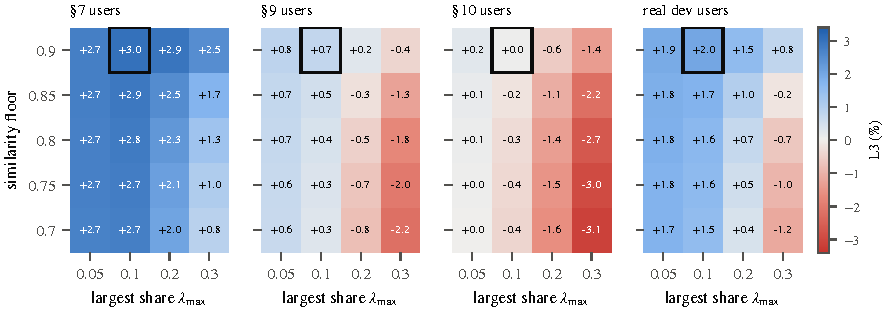
\includegraphics[width=\linewidth]{figures/fig_grids.pdf}
\caption{L3 (\%) over the mixing grid at $\tau = 0.01$ (development probe round 14, one code state for all four user sets).
The framed cell is the app's setting.}
\label{fig:grids}
\end{figure}

\section{Development runs on the \S7 users}\label{app:dev}

\begin{table}[H]
\centering
\small
\caption{App runs with all three arms on the consumed \S7 users while developing the second version and the note forms
(not used for any decision). L1 in points; L2, L2b and L4 as in \cref{tab:registered}; ``stored'': injected mistakes that
reached the memory. $^{a}$Older definition of L5 (tokens per second including the prompt, FK/off).}
\label{tab:dev}
\begin{tabular}{@{}llrllrlrr@{}}
\toprule
Run & Results commit & L1 & L2 F/FK & L2b F/FK & L3 (\%) & L4 F/FK (off) & L5 & stored \\
\midrule
\tablebody{tab_dev}
\bottomrule
\end{tabular}
\end{table}

v2a: note and guard with the old memory filter; v2b: whole-text word check and the grid's mixing setting; v2c: sentence
exclusion on any near-form flag (too strict: L3 fell to 0.53\pct); v2d: sentence exclusion only for confirmed mistakes;
v2e: similarity floor 0.90; v2f: fixes from the third review (the code measured in \S8); v2g: guard against printing the
note; v2h: note as sentences.

\section{Selection of real users}\label{app:selection}

Source: \texttt{allenai/WildChat-1M}, revision \texttt{7d6490e}, the first three of 14 parquet shards. Conversations
labelled English or German and not marked toxic or redacted; user turns in the conversation's language. A user is a
hashed IP address within one language. Messages are kept if they are plain prose (20--300 characters; no code, links or
markup; at most two line breaks; at least 85\pct{} letters and spaces), ordered by conversation time and then turn
identifier, and taken only if not a near copy of an earlier taken message (\texttt{difflib} similarity $< 0.8$). Users
with six such messages qualify: four taught, two held out. Split: development if the first byte of SHA-256(hashed IP) is
even, otherwise test. Qualified pools: development 1{,}504 English and 58 German users; test 1{,}500 and 54. With seed
20261023, 20 users per language were drawn for development and for test (\S11); for \S12, 20 per language from the 1{,}478
English and 34 German test-side users whose hashed IP was in no earlier set (seed 20261025). No user appears in two sets. The selection file
holds, per message, the shard, conversation hash, turn identifier, SHA-256 and length, and was committed (41431d1; \S12:
789abea) before any measurement on these users. Facts were drawn from the pools of the synthetic generator; mistakes and
probes follow the synthetic sets, with a mistake sentence placed on a new line after a real message without closing
punctuation so that it forms a sentence of its own.

\section{Timeline of registrations and measurements}\label{app:timeline}

\begin{table}[H]
\centering
\small
\caption{Commits (UTC, 19 October 2026) that registered each section, triggered its measurement and added its results.
Test users were committed before any measurement on them (\S8: 234bab0; \S9: d405a03; \S10: 9831eed; real users:
41431d1; \S12 users and probes: 789abea); the \S12 cue words were frozen in 96e9897 (18:34).}
\label{tab:timeline}
\begin{tabular}{@{}llll@{}}
\toprule
Section & Registered & Measurement triggered & Results committed \\
\midrule
\S7 & a594d98 (00:28), amended \S7.1--7.4 until 04:36 & 296c62d (04:36) & b12fe09 (04:41) \\
\S8 & b59414a (10:20) & bbfa8e0 (10:21) & 15e59bc (10:29) \\
\S9 & bed30a6 (13:02) & e0685aa, 2917afc (13:02) & 88f7f30 (13:10), b41a222 (13:18) \\
\S10 & 87a4c4d (13:22) & ca923a0 (13:22), 26c5924 (13:23) & 203881f (13:30), 039d25c (13:38) \\
\S11 & 3fb881a (18:10; same commit) & 3fb881a & 975d994 (18:19) \\
\S12 & 789abea (18:38; same commit) & 789abea, e2f3790 (18:38) & 8b4e2fc (18:48), 106956f (18:56) \\
\bottomrule
\end{tabular}
\end{table}

\section{Discrepancies between documents and result files}\label{app:discrepancies}

We report the result files wherever the project's prose documents differ from them. (i) The preregistration's tables for
\S9.1 and \S10.1 gave the off-arm L4 count as 2 and 3; the result files record 1 (\S9) and 2 (\S10), with limits of 3 and
4. No decision changes; both sections now carry a dated correction note. (ii) The model card attributed 10 stored
mistakes to \S10; the result files record 10 for \S8 and 5 for \S10. The model card has been corrected. (iii) Counts of replies that printed the note itself in \S8 cannot be reproduced exactly with the pattern in
the current code, so we do not report them.

\end{document}
